\chapter{Mengenal Kecerdasan Buatan dan Scikit-Learn}
Buku umum yang digunakan adalah \cite{russell2016artificial} dan  
untuk sebelum UTS menggunakan buku \textit{Python Artificial Intelligence Projects for Beginners}\cite{eckroth2018python}.
Dengan praktek menggunakan python 3 dan editor anaconda dan library python scikit-learn.
Tujuan pembelajaran pada pertemuan pertama antara lain:
\begin{enumerate}
\item
Mengerti definisi kecerdasan buatan, sejarah kecerdasan buatan, perkembangan dan penggunaan di perusahaan
\item
Memahami cara instalasi dan pemakaian sci-kit learn
\item
Memahami cara penggunaan variabel explorer di spyder
\end{enumerate}
Tugas dengan cara dikumpulkan dengan pull request ke github dengan menggunakan latex pada repo yang dibuat oleh asisten riset.

\section{Teori}
Praktek teori penunjang yang dikerjakan :
\begin{enumerate}
\item
Buat Resume Definisi, Sejarah dan perkembangan Kecerdasan Buatan, dengan bahasa yang mudah dipahami dan dimengerti. Buatan sendiri bebas plagiat[hari ke 1](10)
\item
Buat Resume mengenai definisi supervised learning, klasifikasi, regresi dan unsupervised learning. Data set, training set dan testing set.[hari ke 1](10)
\end{enumerate}

\section{Instalasi}
Membuka https://scikit-learn.org/stable/tutorial/basic/tutorial.html. Dengan menggunakan bahasa yang mudah dimengerti dan bebas plagiat. 
Dan wajib skrinsut dari komputer sendiri.
\begin{enumerate}
\item
Instalasi library scikit dari anaconda, mencoba kompilasi dan uji coba ambil contoh kode dan lihat variabel explorer[hari ke 1](10)
\item
Mencoba Loading an example dataset, menjelaskan maksud dari tulisan tersebut dan mengartikan per baris[hari ke 1](10)
\item
Mencoba Learning and predicting, menjelaskan maksud dari tulisan tersebut dan mengartikan per baris[hari ke 2](10)
\item
mencoba Model persistence, menjelaskan maksud dari tulisan tersebut dan mengartikan per baris[hari ke 2](10)
\item 
Mencoba Conventions, menjelaskan maksud dari tulisan tersebut dan mengartikan per baris[hari ke 2](10)
\end{enumerate}


\section{Penanganan Error}
Dari percobaan yang dilakukan di atas, apabila mendapatkan error maka:

\begin{enumerate}
	\item
	skrinsut error[hari ke 2](10)
	\item
Tuliskan kode eror dan jenis errornya [hari ke 2](10)
	\item
Solusi pemecahan masalah error tersebut[hari ke 2](10)

\end{enumerate}

\section{Cokro Edi Prawiro/1164069}
\subsection{Praktek teori penunjang}
\begin{enumerate}
\item
Kecerdasan Buatan \textit{Artificial Intelligence} adalah suatu cabang dalam bidang sains komputer yang mengkaji bagaimana untuk melengkapi sebuah komputer dengan kemampuan atau kepintaran saperti manusia. Komputer tersebut di harapkan dapat belajar sendiri dengan cara mengumpulkan data-data yang diterimanya, yang berguna sebagai parameter untuk memecahkan masalah. Jadi kecerdasan buatan merupakan kecerdasan yang di program dalam koputer untuk memecahkan masalah secara tepat dan cepat atau untuk memberikan kemungkinan keberhasilan dan kegagalan pada solusi dari suatu masalah.\par
Adapun kecerdasan buatan menurut para ahli adalah sebagai berikut :
\begin{itemize}
\item 
Kecerdasan Buatan merupakan Kawasan penelitian, aplikasi dan intruksi yang terkait dengan pemerograman komputer untuk melakukan sesuatu hal yang dalam pandangan manusia adalah cerdas (H. A. Simon[1997]).
\item 
Kecerdasan buatan adalah bidang studi yang berhubungan dengan penangkapan, pemodelanm, dan penyimpanan kecerdasan manusia dalam sebuah sistem teknologi sehingga sistem tersebut dapat menfasilitasi proses pengambilan keputusan yang biasanya dilakukan oleh manusia (Haag dan keen[1996]).
\end{itemize}
Sejarah dan Perkembangan Kecerdasan Buatan.\\
ketika \textit{Rene Descartes} mengemukakan gagasan yang menjadi cikal bakal kecerdasan buatan pada abad 17 mengemukakan bahwa hewan bukan apa-apa melainkan hanya mesin yang rumit yang dilanjutkan oleh \textit{Belaise Pascal} yang telah menciptakan mesin penghitung digital mekanis pertama pada tahun 1642. Lalu pada abad 19 \textit{Charles Babbage} dan\textit{Ada lovelace}  bekerja sama membuat mesin penghitung mekanis yang dapat di program.\par
Perkembangan kecerdasan buatan inipun terus berlanjut,\textit{ Bertrand Russell} dan\textit{ Alferd North Whithead} menerbitkan \textit{mathematica}, yang merombak logika formal. Setelah itu dilanjutkan dengan penemuan oleh \textit{ Warren McCulloch} dan \textit{ Walter Pitts} menerbitkan “Kalkulus Logis Gagasan yang tetap ada dalam Aktivitas” pada 1943 yang meletakan pondasi awal berupa jaringan syaraf 
Kemudian pada tahun 1950-an adalah periode awal usaha aktif kecerdasan buatan. Progam Kecerdasan buatan pertama yang bekerja di ciptakan pada tahun 1951 untuk menjalankan mesin Ferranti Mark I di University of Manchester (UK) yaitu sebuah program permainan naskah yang ditulis oleh \textit{Christoper Strachey} dan program permainan catur yang ditulis oleh \textit{Dietric Prinz}. Kemudian pada konferensi pertama tahun 1956  \textit{John McCarthy} mengemukakan istilah “kecerdasan buatan” kemudian dia juga menemukan bahasa pemerograman lips. \textit{Joseph Weizenbaum}  menciptakan ELIZA, sebuah chatterbot yang menerapkan psikoterapi Rogerian.\par
Selama rentang waktu tahun 1960-an dan 1970-an, \textit{Joel Moses}  mendemonstrasikan kekuatan pertimbangan simbolis untuk mengintegrasikan masalah di dalam program Macsyma, yang merupakan program yang pertamakali sukses dalam bidang matematika. Kemudian pada tahun 1980-an industry kecerdasan buatan ini berkembang walu sudah di mulai pada tahun 1970-an Evolusi kecerdasan buatan berjalan dalam dua jalur yang berbeda yaitu meniru proses berpikir manusia untuk menyelesaikan masalah umum. Kedua mengkombinasikan pemikiran terbaik para ahli pada sepotong software yang dirancang untuk memecahkan persolalan yang spesifik. 

\item
Supervised learning adalah sebuah pendekatan dengan syarat sudah terdapat data yang dilatih kemudian harus terdapat variable yang ditargetkan sehingga tujuan dari pendekatan ini adalah pengelompokan data terhadap data yang telah ada. Ciri khas dari Supervised learning yaitu terdapat label atau nama kelas pada data latih (supervisi) dan data baru di klasifikasikan berdasarkan data latih. Data latih sikelompokan berdasarkan ukuran kemiripan pada suatu kelas. Berdasarkan keluaran dari fungsi, Supervised learning dibagi menjadi 2, regresi dan klasifikasi. Regresi terjadi jika output dari fungsi merupakan nilai yang kontinyu, sedangkan klasifikasi terjadi jika keluaran dari fungsi adalah nilai tertentu dari suatu atribut (tidak kontinyu). Tujuan dari Supervised learning adalah untuk memprediksi nilai dari fungsi untuk sebuah data masukanyang sah setelah melihat sejumlah data latih\cite{februariyanti2012klasifikasi}.\\
Adapun pengertian klasifikasi dan regresi adalah sebagai berikut :
\begin{itemize}
\item
Klasifikasi merupakan pengelompokan berdasarkan parameter tertentu yang tidak konstan contoh pada mahluk hidup yaitu persamaan ciri cara hidup dan tempat hidup.
\item
Regresi yaitu pengeluaran nilai output yang konstan jika dipicu dengan parameter tertentu biasanya regresi disini berbentuk regresi linier. Regresi linier yaitu metode statistika yang digunakan untuk membentuk model hubungan antara variabel terikat(dependen,respon,Y) dengan satu atau lebih variabel bebas(independent, prdiktor, X). Apabila banyaknya variabel bebas hanya ada satu, disebut sebagai regresi linier sederhana, sedangkan apabila terdapat lebih dari satu variabel bebas, disebut sebagai regresi linier berganda \cite{kurniawan2008regresi}.
\end{itemize}
unsupervised learning adalah pendekatan yang tidak memerlukan data latih atau data training untuk melakukan prediksi atau klasifikasi. Berdasarkan model secara matematisnya, algoritma ini tidak memiliki target variabel. Tujuan dari algoritma ini yaitu pengelompokan objek yang memiliki kesamaan atau hampirsama dalam satu cakupan wilayah tertentu. Kemudian pada unsupervised learning tidak terdapat label atau nama kelas pada data latih.
Kemudian dataset merupakan objek yang menggambarkan data itu sendiri dan relasinya di memory. Struktur datanya mirip dengan struktur data di basisdata. Jadi strikturnya terdiri atas baris kolon dan juga ada sejenis relasi data. Pada dataset terdiri bagian bagian yaitu tranning set dan Testing set.
Adapun pengertian dari tranning set dan Testing set adalah sebagai berikut :
\begin{itemize}
\item
Training set adalah bagian dari dataset itu sendiri yang dilatih untuk membuat prediksi atau algoritma mesin learning lainnya sesuai keinginan atau tujuan data itu dibuat.
\item
Testing set adalah bagian dari dataset yang di tes atau diujicoba untuk melihat keakuratannya dengan katalain melihat peformanya.
\end{itemize}
\end{enumerate}

\subsection{Instalisasi}\par
Pada proses instalisasi ini langkah pertama yaitu mengakses website scikit dengan mengakses link berikut  https://scikit-learn.org/stable/tutorial/basic/tutorial.html maka hsilnya dapat dilihat pada gambar \ref{sc} kemudian setelah itu klik button installation maka akan muncul tampilan yang dapat dilihat pada gambar \ref{sc1}.
\begin{figure}[ht]
      \centerline{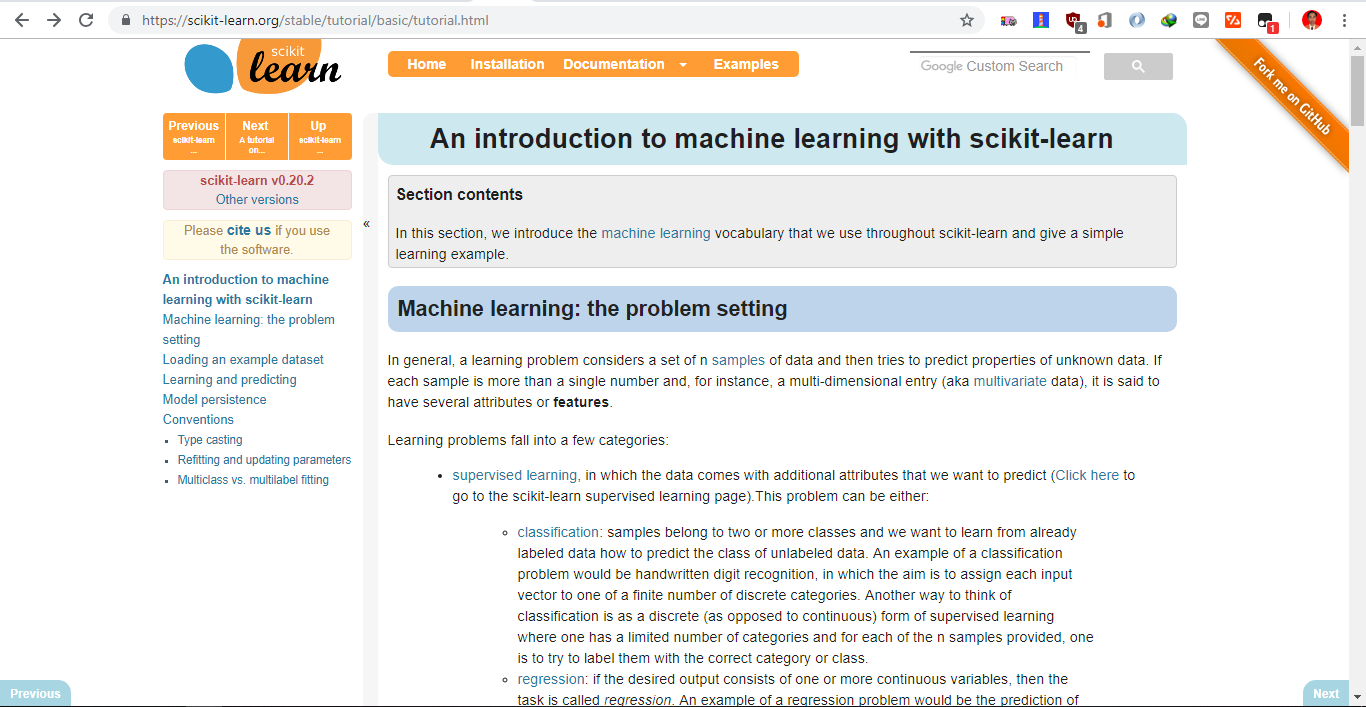
\includegraphics[width=1\textwidth]
      {figures/sc}}
      \caption{Tampilan website Scikit 1.}
      \label{sc}
      \end{figure}
\begin{figure}[ht]
      \centerline{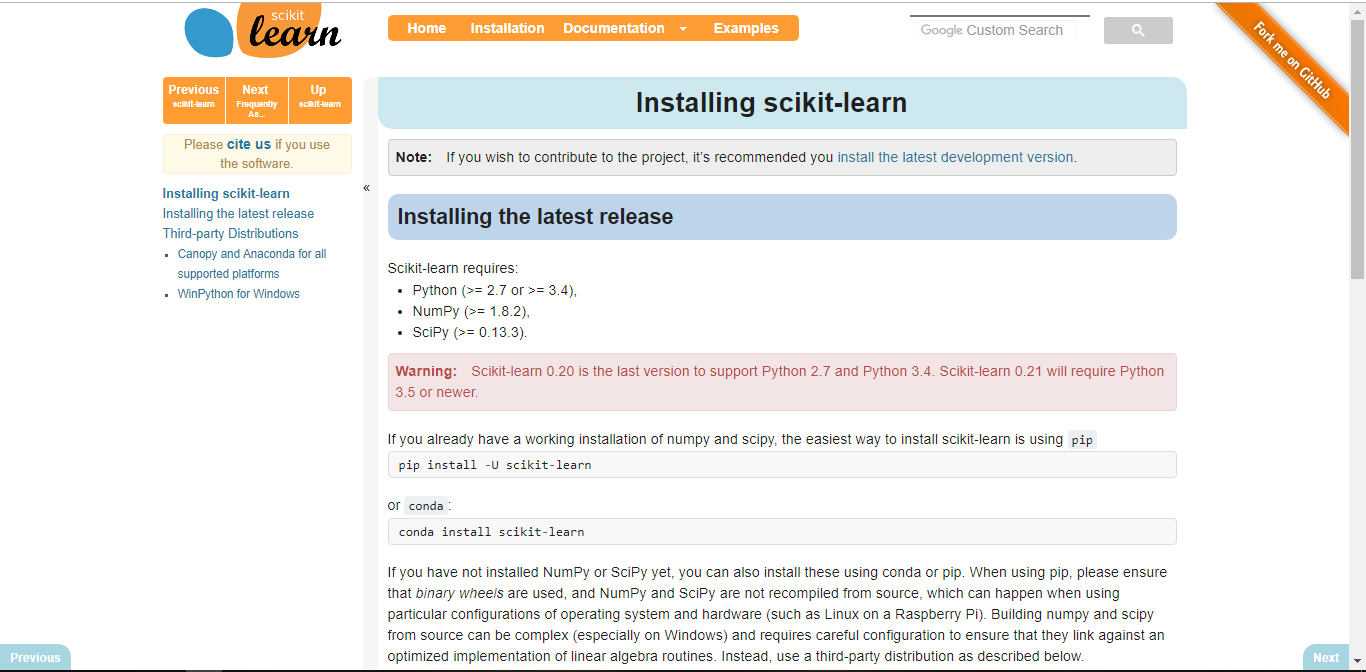
\includegraphics[width=1\textwidth]
      {figures/sc1}}
      \caption{Tampilan website Scikit 2.}
      \label{sc1}
      \end{figure}
\begin{enumerate}
\item 
cara instalisasi Instalasi library scikit dari anaconda langkah pertama instal terlebih dahulu anacondanya dikarenakan anaconda sudah include dengan python maka codingan python dapat digunakan di anaconda dan ketika diperikas versinya maka akan muncul tampilan seperti Gambar \ref{c}
\begin{figure}[ht]
      \centerline{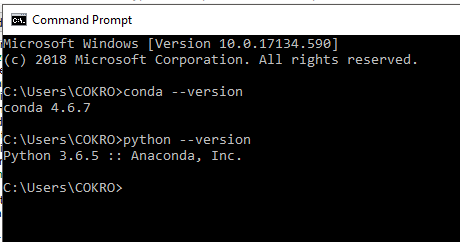
\includegraphics[width=1\textwidth]
      {figures/c}}
      \caption{Tampilan Versi Python dan Anaconda .}
      \label{c}
      \end{figure}
kemudian pada cmd administrator install library sikic dengan cara memasukan codingan pip install -U scikit-learn maka hasilnya seperti seperti pada gambar \ref{c1} berikut.
\begin{figure}[ht]
      \centerline{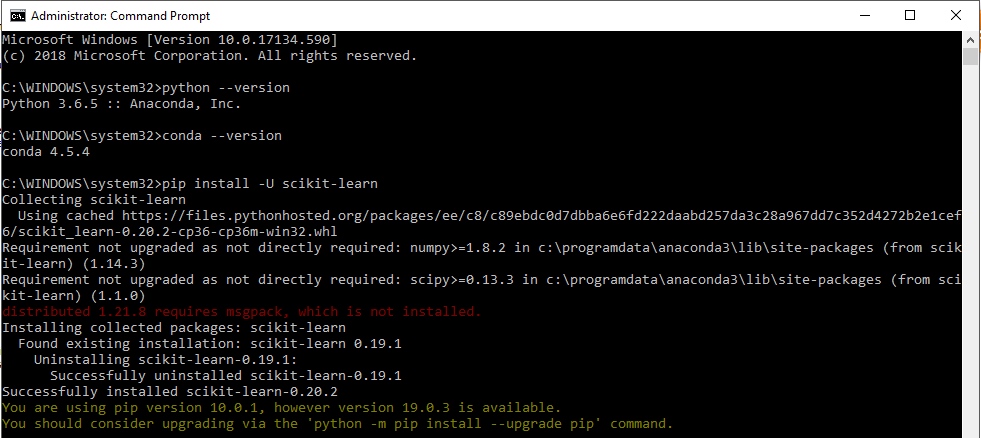
\includegraphics[width=1\textwidth]
      {figures/c1}}
      \caption{Instalisasi Library Sikic.}
      \label{c1}
      \end{figure}
setelah itu masukan kembali perintah berikut di cmd conda install scikit-learn jika hasilnya seperti pada gambar \ref{c2} maka librari sikic telah teristal dan siap untuk di gunakan.
\begin{figure}[ht]
      \centerline{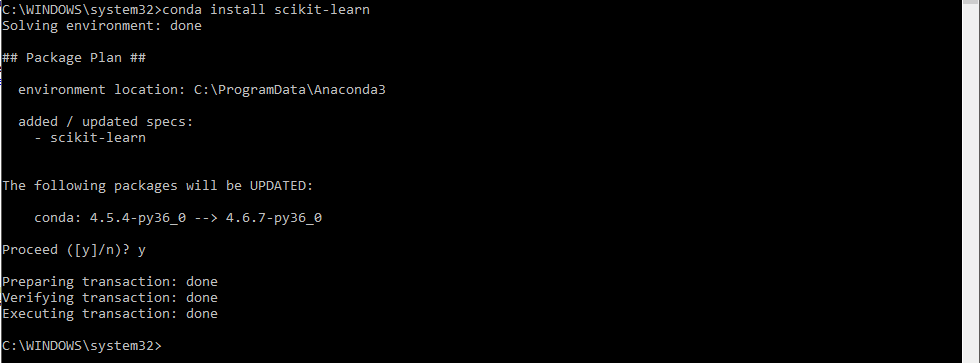
\includegraphics[width=1\textwidth]
      {figures/c2}}
      \caption{.}
      \label{c2}
      \end{figure}
kemudian untuk mencobanya tuliskan perintah python pada cmd lalu masukan codingan print("Hello Anaconda!") maka hasilnya terlihat seperti gambar \ref{c3} codingan print("Hello Anaconda!") yaitu berfungsi mencetak nilai yang ada di dalam kurung dan di antara kutip.
\begin{figure}[ht]
      \centerline{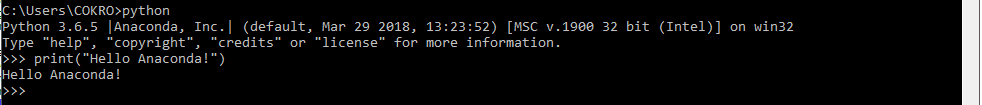
\includegraphics[width=1\textwidth]
      {figures/c3}}
      \caption{.}
      \label{c3}
      \end{figure}

\item
cara mencoba dataset yaitu dengan cara memasukan perintah berikut pada cmd seperti pada gambar \ref{c4} 
\begin{figure}[ht]
      \centerline{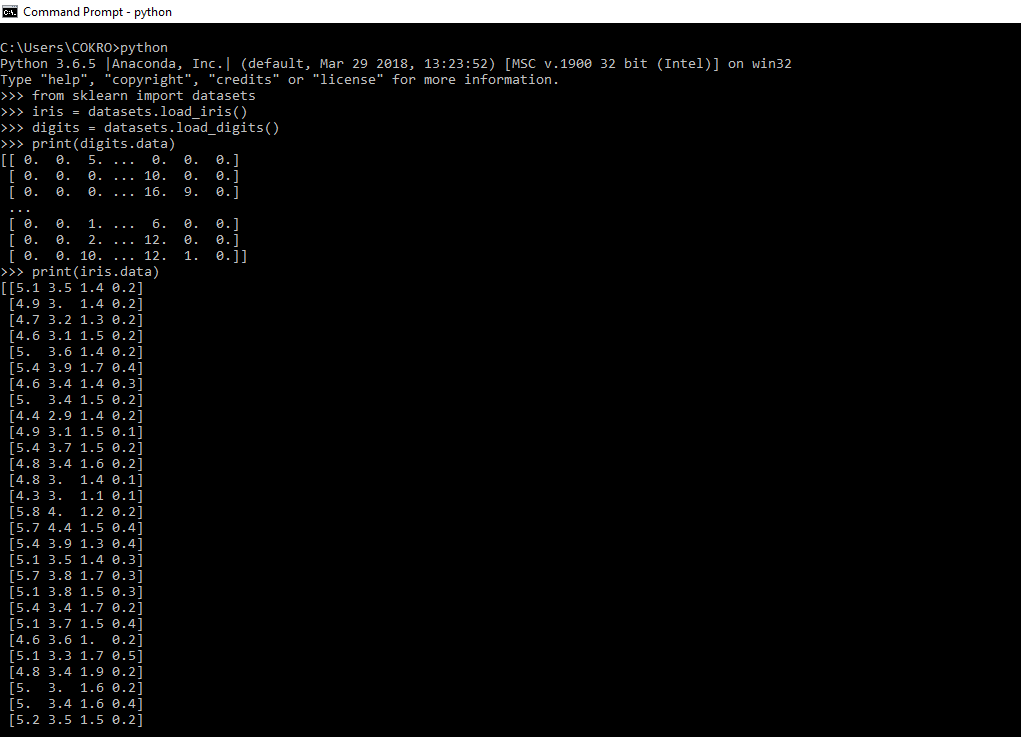
\includegraphics[width=1\textwidth]
      {figures/c4}}
      \caption{I.}
      \label{c4}
      \end{figure}
\begin{itemize}
\item
pada codingan from sklearn import datasets menjelaskan inport librari dataset dari librari sikic pada gambar \ref{c4}
\item
pada codingan iris = datasets.load iris iris beearti parameter atau acuan bernama iris kemudian di load ke dalam dataset sebagai perbandingan kalau daram diagram iris bisa disebut X nya pada gambar \ref{c4}
\item 
pada codingan digits = datasets.load digits digits berarti parameter hampir mirip seperti iris tadi namun digits merupakan kebalikannya kalau di dalam diagaram dia bernilai Y pada gambar \ref{c4}
\item
kemudian pada codingan print(digits.data) yaitu mencetak data digits yang di bandingkan dengan data iris pada gambar \ref{c4}
\item 
pada codingan print(iris.data) yaitu mencetak data iris yang dibandingkan dengan data digits pada gambar \ref{c4}
\end{itemize}
\end{enumerate}
